%----------------------------------------
%   PREAMBLE
%----------------------------------------

\documentclass[12pt,a4paper]{article}

\usepackage{multicol,lipsum, multirow}
\usepackage[a4paper, left=20mm, top=20mm, right=20mm, bottom=20mm,footskip=0.4in]{geometry}

%% Language and font encodings
\usepackage[english]{babel}
\usepackage[utf8x]{inputenc}
\usepackage[T1]{fontenc}

\usepackage{mathptmx}

\usepackage{sectsty}
\sectionfont{\fontsize{12}{13}\selectfont}
\subsectionfont{\fontsize{12}{13}\selectfont}
\usepackage[labelfont={bf,sf,footnotesize,singlespacing},textfont={sf,footnotesize,singlespacing},singlelinecheck=false,margin=0pt]{caption} % format captions
\usepackage{tabu}
\usepackage[backend=biber, style=nature, citestyle=numeric-comp, sorting=none]{biblatex}
\addbibresource{references.bib}
\renewcommand*{\bibfont}{\fontsize{11}{12}\selectfont}
\usepackage{authblk} % authors & affiliations
\usepackage[british]{babel} % localised formatting
\usepackage[colorlinks,linkcolor=black,citecolor=black,urlcolor=black]{hyperref} % clickable links
\usepackage{subcaption} % for subfigures
\usepackage[labelfont={bf,footnotesize,singlespacing},textfont={it,footnotesize,singlespacing},justification={centering},singlelinecheck=false,margin=0pt]{caption} % format captions
\usepackage{chemformula} % does what it says on the tin
\usepackage{csvsimple} % auto-table CSV files
\usepackage{longtable} % multi-page tables
\usepackage{multirow} % multi-rows in tables
\usepackage{tabularx} % auto-wrap lines in tables
\usepackage{wrapfig} % wrap text around figures
\usepackage{float} 
\usepackage[separate-uncertainty=true,mode=text]{siunitx} % number and unit
\usepackage{lscape} % landscape pages for tables
\usepackage{pdflscape} % show those pages the right way round in PDF viewers
\usepackage{nomencl} % nomenclature fun
    \makenomenclature
    \newcommand{\nomunit}[1]{\renewcommand{\nomentryend}{\hspace*{\fill}#1}}
\usepackage{amsmath} % align equations
\usepackage{tabularx} % split table columns equal.
\usepackage{gensymb} % for degree symbols
\usepackage[compact]{titlesec} % reduces spacing after headings
    \titlespacing{\section}{0pt}{0.5ex}{0ex}
    \titlespacing{\subsection}{0pt}{0.2ex}{0ex}
    \titlespacing{\subsubsection}{0pt}{0ex}{0ex}   
\usepackage{makecell} % for forcing line breaks inside cells
\usepackage{graphicx} % make images work  
\usepackage{url} % references in url
\usepackage{booktabs}
\usepackage{tikz} % for control system block diagrams
    \usetikzlibrary{shapes,arrows}
    \usetikzlibrary{calc}
\usepackage{enumitem}
\setitemize{noitemsep}
\setlist[itemize]{noitemsep, topsep=0pt, leftmargin=*} %reduces spacing in between items
\setlist[enumerate]{noitemsep, topsep=0pt, leftmargin=*} %reduces spacing in between enumerate
\usepackage[nottoc,numbib]{tocbibind} %add bibiliography into toc

\usepackage{pdfpages}
\usepackage{xcolor} % Required for specifying custom colours
\definecolor{paleBlue}{RGB}{207, 244, 255} % Colour of the box
\definecolor{GoodGreen}{RGB}{180, 237, 210}
\definecolor{DeepPurple}{RGB}{148,51,106}
\definecolor{LightPurple}{RGB}{195, 144, 209}
\definecolor{PurplyBlue}{RGB}{172, 172, 222}
\definecolor{Blue}{RGB}{171, 218, 252}
\definecolor{LightAqua}{RGB}{229, 252, 255}


\usepackage{color, colortbl}
\overfullrule=0mm %removed black boxes <idk why> - James
\usepackage{setspace}

%----------------------------------------
%   REPORT CONTENTS
%----------------------------------------
\begin{document}

%Coverpage
\includepdf[pages=1,scale=1.128]{CoverPage}

\singlespacing

%ToC
\newpage
\pagenumbering{roman}
\tableofcontents

%nomenclature
\newpage
\addcontentsline{toc}{section}{Nomenclature}
\label{nomenclature}

%Example Nomenclature
\newpage
\nomenclature{$T$}{Temperature \nomunit{\si{K}}}
\nomenclature{$x_{tol}$}{Conversion of Toluene \nomunit{\si{-}}}
\nomenclature{$\rho_{c}$}{Density of Catalyst \nomunit{\si{g \cdotp m^{-3}}}}
\nomenclature{$\epsilon$}{Void Fraction of Catalyst \nomunit{\si{-}}}
\printnomenclature
\newpage

% import sections
\onecolumn
\setlength{\parskip}{3pt} % paragraph spacing 
\setlength{\parindent}{0pt} % no paragraph indent
{\fontfamily{lmss}\selectfont %helvetica font
\pagenumbering{arabic}
% Separator Design Section = 10 marks out of 100
% Choice of Separator (3 marks)
% Separator Modelling (5 marks)
% Physical Design (2 marks)
% Max 20 pages 
% Table of Contents, Nomenclature and References are not included in the page limits

% Additional Support Material such as key Aspen, gPROMS, Excel spreadsheets or other programmes should be delivered in digital form and sent in compressed format (zipped) to the Co-ordinator
% Need to prepare design data sheet of process equipment (refer to Supporting Documentation LaTeX)

\section{Introduction}
\label{sec:introduction}

\begin{itemize}
    \item Emphasise why separations is important, especially when we want to reach such high purities (especially within the pharmaceutical industry)
    \item Mention an outline of our (hopefully) novel / innovative design and the objective of this separation (purity, isomers, brief economic / environmental considerations)
    \item 1-2 sentences explaining our approach in obtaining our detailed design 
    \item 1 sentence saying what this report outlines (the design methods & our findings)
\end{itemize}




%Example citation
This is an example citation \cite{Caliman}

\section{Selection of the Detailed Design}
\label{sec:design_selection}

% HOW THINGS WERE DECIDED 
% Choice of separator:
% a) Why is this separation crucial in the overall process 
% b) How did you choose the type of process? What, if any, alternatives were considered and why were they rejected?
% c) are there any novel or especially difficult aspects to the separation

\begin{itemize}
    \item Explain why crystallisation is the crucial step in our entire separation process - our USP is the higher-than-average cis:trans ratio as well as a very high promised purity - crystallisation is essential to achieve these goals 
    \item Explain the feed coming out of final reactor for both permethrin and cypermethrin (include a brief sentence about decanter & flash being required before crystallisation even though it's not part of the detailed design but it's still the same step)
    \item Impurities remain in the system along with the desired product, permethrin and cypermethrin - permethrin stream is exactly the same as what exits final reactor
    \item Due to the desire to sell to both the pharmaceutical and agricultural sectors of industry, the minimum purity has to be at least xx\% to be sold to the former
    \item To finalise the overall separation system to obtain xx\% and xx\% purity permethrin and cypermethrin respectively as products, a combination of techniques were employed.
\end{itemize}
% WHAT WAS DECIDED AND WHY (have more why when writing)

\subsection{Selection of Employed Separation Technique}
\begin{itemize}
    \item Traditionally, pharmaceutical processes often employ crystallisation, chromatography, distillation and filtration in order to meet the high purities specified by regulations
    \item A high final purity was required, due to the desire to sell to both the agricultural and pharmaceutical segments simultaneously (another aspect of modularity!) 
    \item Straight forward separations such as a large difference in boiling points = distillation column but conducted Jaksland analysis on several less straight forward steps of the separation process to find feasible separation pathways, including this step (may want to include a table of key properties for this decision)
    \item final decision between crystalliser and precipitator (precipitator advantages = almost instantaneous, high likelihood of oiling out, easy to separate and no seeding required, however due to this there is no separation between cis and trans and a larger energy consumption as more water is required for the system which is difficult to separate from methanol) 
    \item This resulted in crystallisation being favoured as the final step (also modularity enforced due to the similar melting points of both permethrin and cypermethrin and want to take advantage of this)
    \item Other techniques considered were chromatography but this is cost-intensive with intense solvent consumption as well as difficult to scale-up to commercial/industrial levels. Distillation was not picked due to smaller difference in boiling points, moreover there was a high possibility of thermal decomposition of the product at the temperatures that would have been used. An additional consideration was the possibility of enantiomer switching and want to avoid trans becoming cis, however this risk was deemed low, especially at the temperatures considered in the entire final separation sequence. Membranes are an attractive option for clean, energy efficient separation however membrane liquids are often instable over long periods of time and require several stages to reach high purities - also risk of membrane fouling
   \item Crystallisation was deemed the most favoured technique due to the following advantanges: ... 
\end{itemize}

\subsection{Detailed Design Separation Units (change title)}
\label{sec:detailed_sep_unit}
\begin{itemize}
    \item Modularity considerations 
    \item Findings from patents, what they showed & how we incorporated / modified them (briefly)
    \item The units which make up our crystalliser design ( crystalliser modelled as 3 continuous stirred tanks with each stage at a different temperature to follow the solubility curve, followed by a filter to remove the solid product with the liquid stream going on to two distillation columns to separate water and methanol from the impurities in the first one and the separation of water and methanol in the second (azeotrope considerations?) recyling both MeOH and H2O to their respective CSTs)
    \item  Detailed design conducted on xx part (if not all). Mechanical design also carried out on this unit.
    \item Making crystallisation continuous 
    \item Any novel/especially difficult aspects of design
    \end{itemize}
    
\subsubsection{Selection of Solvent}

Format table correctly, ensure it matches with other tables - check if headings should capitalise each word & caption table

Considered a greener alternative for methanol as the solvent (ich class 2), however it proved to be the best choice after holistically looking at multiple solvents. Deciding factors with heaviest weightings are solubility and the formation of an azeotrope with water as this will make solvent recovery and separation for recycle more difficult further downstream (requiring azeotropic distillation, additionally more energy-intensive). The toxicity \& environmental concerns associated with methanol were decidedly outweighed by its no azeotrope formation as well as the fact that none of the considered solvents proved to have a distinct advantage (e.g. all similar ratings in terms of safety and environment).  

\begin{table}[h]
\begin{tabular}{cccccccc}
\hline
\multicolumn{1}{|c|}{Solvent}     & \multicolumn{1}{c|}{\begin{tabular}[c]{@{}c@{}}Solubility \\ Parameter\\ (MPa^{1/2})\end{tabular}} & \multicolumn{1}{c|}{\begin{tabular}[c]{@{}c@{}}Binary Water\\  Azeotrope\end{tabular}}                                & \multicolumn{1}{c|}{\begin{tabular}[c]{@{}c@{}}Environmental\\ Considerations\end{tabular}} & \multicolumn{1}{c|}{\begin{tabular}[c]{@{}c@{}}Safety\\ Considerations\end{tabular}} & \multicolumn{1}{c|}{\begin{tabular}[c]{@{}c@{}}Boiling \\ Point (K)\end{tabular}} & \multicolumn{1}{c|}{\begin{tabular}[c]{@{}c@{}}ICH \\ Class\end{tabular}} & \multicolumn{1}{c|}{\begin{tabular}[c]{@{}c@{}}Molecular \\ Weight\end{tabular}} \\ \hline
\multicolumn{1}{|c|}{Methanol}    & \multicolumn{1}{c|}{29.6}                                                                      & \multicolumn{1}{c|}{none}                                                                                             & \multicolumn{1}{c|}{FILL IN}                                                                & \multicolumn{1}{c|}{Health (2), Flammability (3), physical hazard (0)}               & \multicolumn{1}{c|}{337.85}                                                       & \multicolumn{1}{c|}{2}                                                    & \multicolumn{1}{c|}{32.04}                                                       \\ \hline
\multicolumn{1}{|c|}{Ethanol}     & \multicolumn{1}{c|}{26.5}                                                                      & \multicolumn{1}{c|}{\begin{tabular}[c]{@{}c@{}}Boils at 78.2 C, volume composition\\ of 95\% alcohol\end{tabular}}    & \multicolumn{1}{c|}{}                                                                       & \multicolumn{1}{c|}{Health (2), Flammability (3), physical hazard (0)}               & \multicolumn{1}{c|}{351.55}                                                       & \multicolumn{1}{c|}{3}                                                    & \multicolumn{1}{c|}{46.07}                                                       \\ \hline
\multicolumn{1}{|c|}{Propanol}    & \multicolumn{1}{c|}{24.5}                                                                      & \multicolumn{1}{c|}{\begin{tabular}[c]{@{}c@{}}Boils at 87.7 C, volume composition\\ of 71.7\% alcohol\end{tabular}}  & \multicolumn{1}{c|}{}                                                                       & \multicolumn{1}{c|}{Health (1), Flammability (3), physical hazard (0)}               & \multicolumn{1}{c|}{370.45}                                                       & \multicolumn{1}{c|}{3}                                                    & \multicolumn{1}{c|}{60.1}                                                        \\ \hline
\multicolumn{1}{|c|}{Isopropanol} & \multicolumn{1}{c|}{23.5}                                                                      & \multicolumn{1}{c|}{\begin{tabular}[c]{@{}c@{}}Boils at 80.4\%, volume composition \\ of 87.7\% alcohol\end{tabular}} & \multicolumn{1}{c|}{}                                                                       & \multicolumn{1}{c|}{Health (1),   Flammability (3), Instability (0)}                   & \multicolumn{1}{c|}{355.65}                                                       & \multicolumn{1}{c|}{3}                                                    & \multicolumn{1}{c|}{60.1}                                                        \\ \hline
\multicolumn{1}{l}{}              & \multicolumn{1}{l}{}                                                                           & \multicolumn{1}{l}{}                                                                                                  & \multicolumn{1}{l}{}                                                                        & \multicolumn{1}{l}{}                                                                 & \multicolumn{1}{l}{}                                                              & \multicolumn{1}{l}{}                                                      & \multicolumn{1}{l}{}                                                            
\end{tabular}
\end{table}
    
\subsubsection{Selection of Crystalliser}
%not sure if this should go under "selection of separation technique" or slightly more above - shouldn't end this section with this basically 

   \begin{itemize}
  %remember to relate back to our specific compounds and to our case in particular, think it would be good to have a key properties table so we can refer to it a couple times 
    \item Once continuous crystallisation was deemed to be the best separation technique, many types of crystallisation were considered and cooling crystallisation using antisolvent seeding was determined to be the optimal scenario. This is due to ... 
    \item Other types of crystallisation considered include a melt crystalliser although the likelihood of fouling is significant since the system is still highly viscous. Evaporative crystallisation was not picked since methanol's boiling point is higher than permethrin's melting point.
    \end{itemize}
    


\section{Looped MSMPR Crystalliser Modelling}
\label{sec:sep_modelling}
%Key Questions / criteria: 
% a) Clearly state the separator design sepcifications / objectives
% b) Detail your design calculations / modelling 
% c) Include sources & reliability of equilibrium and/or kinetic data used 
% d) If thermodynamic/kinetic models have been used, how have they been validated 
% e) How have you allowed for uncertainty in the modelling?
% f) What are the conclusions of the modelling?

TRL --> milling \& MSMPR (both industrially available)\\
Looping method very novel

\subsection{Solubility Estimations}
Solubility equation - use handbook of industrial crystallisation to explain how we arrived at our equation \& any assumptions involved.

\subsubsection{Activity Coefficient Estimations}
\begin{itemize}
    \item Explain/ mention some most commonly used models in pharma (NRTL, Unifac, CosmoSac, Hansen, NRTLSac)
    \item Justify why we used NRTL for activity coeff (takes into account non-ideality in liquid phase - water \& methanol mixing is non-ideal due to the presence of interactions like hydro[hobicity and hydrophilicity)
    \item input, write and briefly explain NRTL equations 
    \item maybe briefly point out/mention that solutes had the same coefficients as activity coefficient is a weak function of temperature but largely a function of composition and solutes were all present in small amounts compared to the solvents
    \item assumed for cypermethrin that cis and trans activity coefficient are the same (this was proven to be the case for permethrin as well as all solutes had the same - tie into bullet above)
\end{itemize}

\subsubsection{Enthalpy of Fusion Estimation}
\begin{itemize}
\item Jobak method since no other way.
\item Melting temperatures mostly from literature (maybe move this to an above section) apart from trans cypermethrin (do group contribution on this).
\item Distinguish and justify the differences in physical properties (enthalpy of fusion as well as melting point) between cis and trans for both cypermethrin and permethrin, backed up by literature (Klaus will want this.)
\end{itemize}

\subsubsection{Melting Point Estimation}
\begin{itemize}
\item Difference in boiling temperature between cis and trans is due to the dipole-dipole and London dispersion forces.
\item Cis is a polar molecule due to the position of group on the same side (non-symmetrical) and therefore has larger IMF
\item Larger IMF \textrightarrow more heat needed to for bond breakage \textrightarrow higher BP
\item Trans pack more efficiently in solid, therefore freezing easier, arrange easier, higher melting point (higher melting point means easier to freeze)
\end{itemize}

\subsubsection{Solubility Curves}
How does solubility curve modelling differ for antisolvent addition and seeding? \\
How did we account for this? \\
How did we account for any errors? \\ What assumptions did we make?

\subsubsection{MSMPR Assumptions}
\begin{itemize}
\item Continuous, steady flow and steady state
\item Perfect mixing of magma
\item No classification of crystals
\item Uniform degree of supersaturation of magma
\item No crystals in feed
\item No crystal breakage
\item Uniform temperature
\item Mother liquor in product magma is equilibrium with crystals
\item Nucleation rate is constant, uniform and due to secondary nucleation by crystal product
\item PSD is uniform for the crystalliser and equal to that in magma
\item All crystals have the same shape
\end{itemize}

\subsection{Seeding Considerations (move section to appropriate place)} 
\begin{itemize}
    \item "In'house" seeding process to obtain the seeds needed for selective crystallisation to separate the cis and trans
    \item Using HPLC chromatography to separate the four isomers of both cis and trans cypermethrin respectively to get a small proportion of very pure isomer - this is then placed into mother liquid and allowed to grow in a batch reactor. Once it has reached a suitable size (put amount), this is then crushed and placed back in the mother liquid and the process is repeated until the 8 separate isomers seeds are suitable for our crystallisation process
    \item For permethrin, both cis and trans seeds will be bought in small quantities. 
\end{itemize}

\newpage
\printbibliography[heading=bibnumbered,title={References}]

% import appendices
\newpage
\appendix
\addcontentsline{toc}{part}{Appendices}

\newpage
\part*{Appendices}
\section{Appendix Section One}
\label{app:appendix-section-one}

%Example Table
\begin{table}[H]
\centering
\caption{\textit{Preliminary reactor specifications}}
\begin{tabular}{|c|c|c|c|c|c|}
\hline
\centering 
\textbf{Code}   & \textbf{Process Equipment} & \textbf{T (K)} & \textbf{P (bar)} & \textbf{Rating (kW)} & \textbf{Estimated Size (L)} \\
\hline
RX101& Packed Bed Reactor & 353.15 & 1.01325 & -16.31 & 1542.26\\
\hline
RX102 & CSTR & 271.15 & 1.01325 & -24.43 & 3303.29 \\
\hline 
RX103 & CSTR & 298.15 & 1.01325 & -5.53 & 1471.69 \\
\hline 
RX104 & Neutralisation Reactor & 298.15 & 1.01325 & -17.81 & 315.13 \\
\hline 
RX105 & Bubble Column Reactor & 293.15 & 1.01325 &-5.35 &  709.71\\
\hline
RX106 & CSTR & 303.15 & 1.01325 & -0.66 & 132.60 \\
\hline
RX107 & CSTR & 289.15 & 1.01325 & -33.51 & 65.50 \\
\hline
RX108 & Bubble Column Reactor & 353.15 & 1.01325 & -4.27 & 481.70 \\
\hline 
\end{tabular}
\centering
\label{table:reactor_specs}
\end{table}


%Example Figure
\begin{figure} [H]
     \centering
     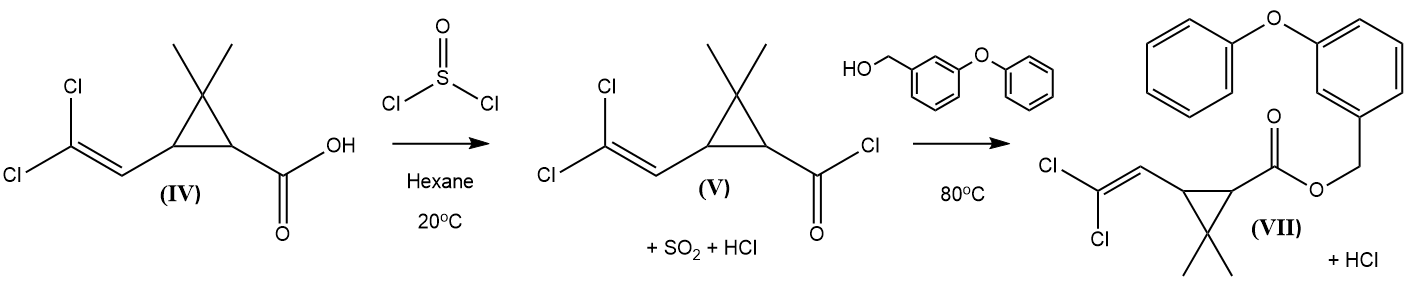
\includegraphics 
     [width=\linewidth]{figures/Permethrin.PNG}
     \caption{\textit{Permethrin reaction pathway adapted from UPL}}
     \label{fig:permethrin_process}
\end{figure}
}
\end{document}